\begin{figure}[ht!]
        \centering                     
        \footnotesize
    \setlength\tabcolsep{2pt}
    \vspace{-0.5in}
    \begin{tabular}{cccc}
        \textbf{\bdraw-350M} & \textbf{\bdraw-750M} & \textbf{\bdraw-3B} & \textbf{\bdraw-20B} \\[2mm]

        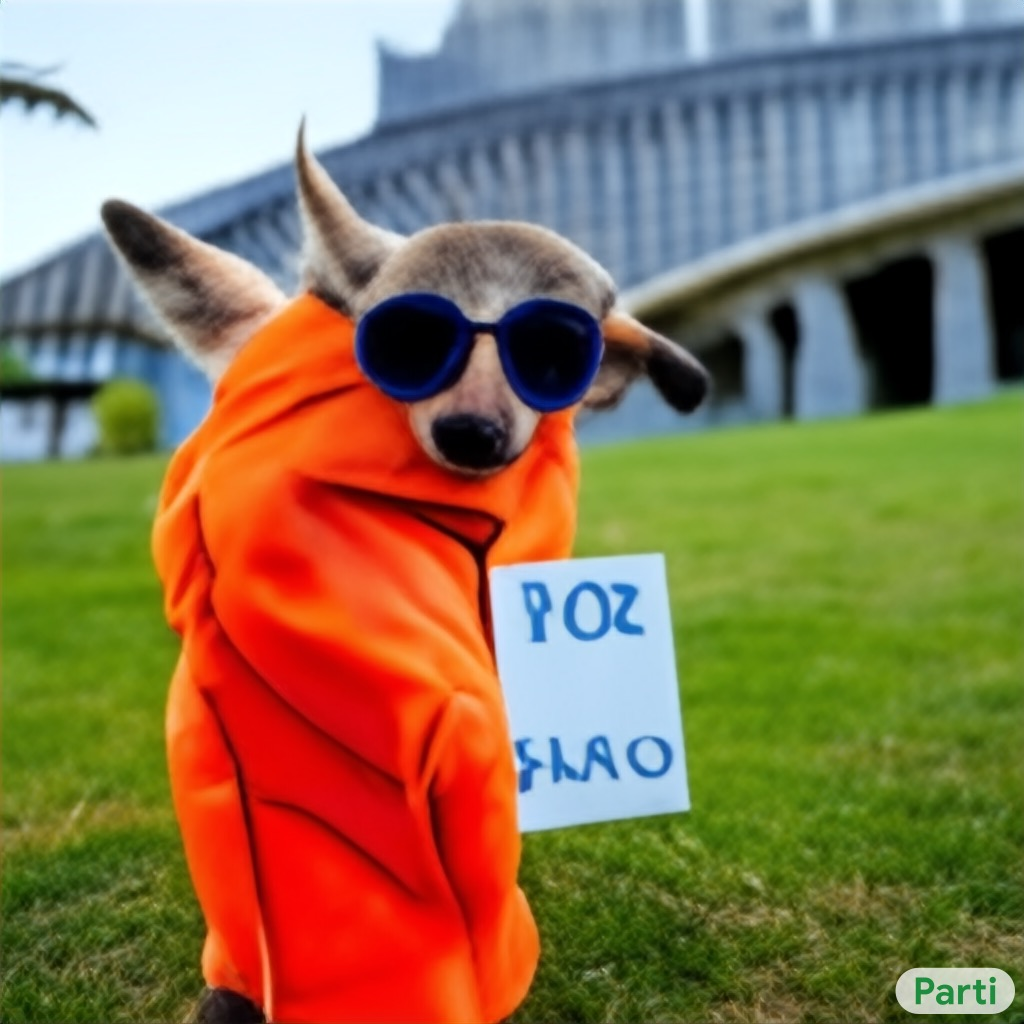
\includegraphics[width=0.24\textwidth]{figures/scaling_comparison/kangaroo_0.jpg} &
        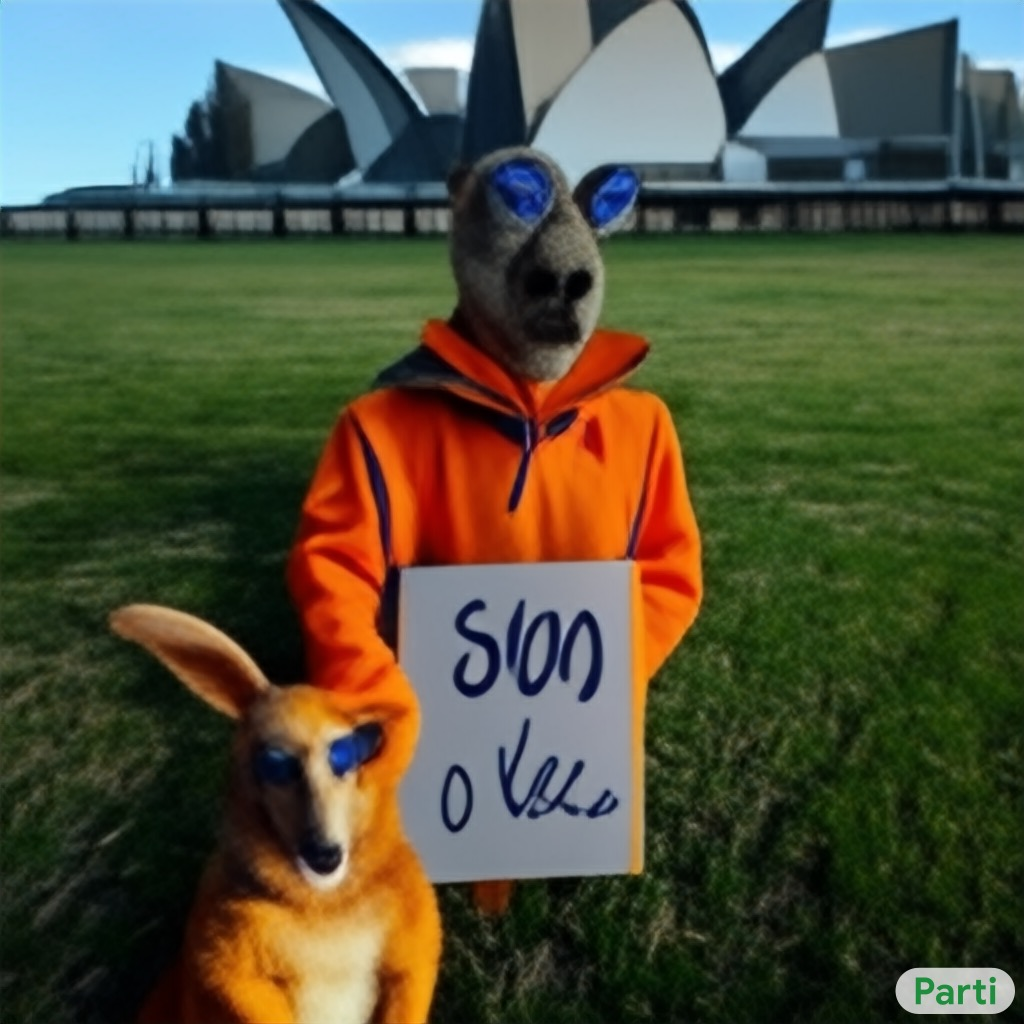
\includegraphics[width=0.24\textwidth]{figures/scaling_comparison/kangaroo_1.jpg} &
        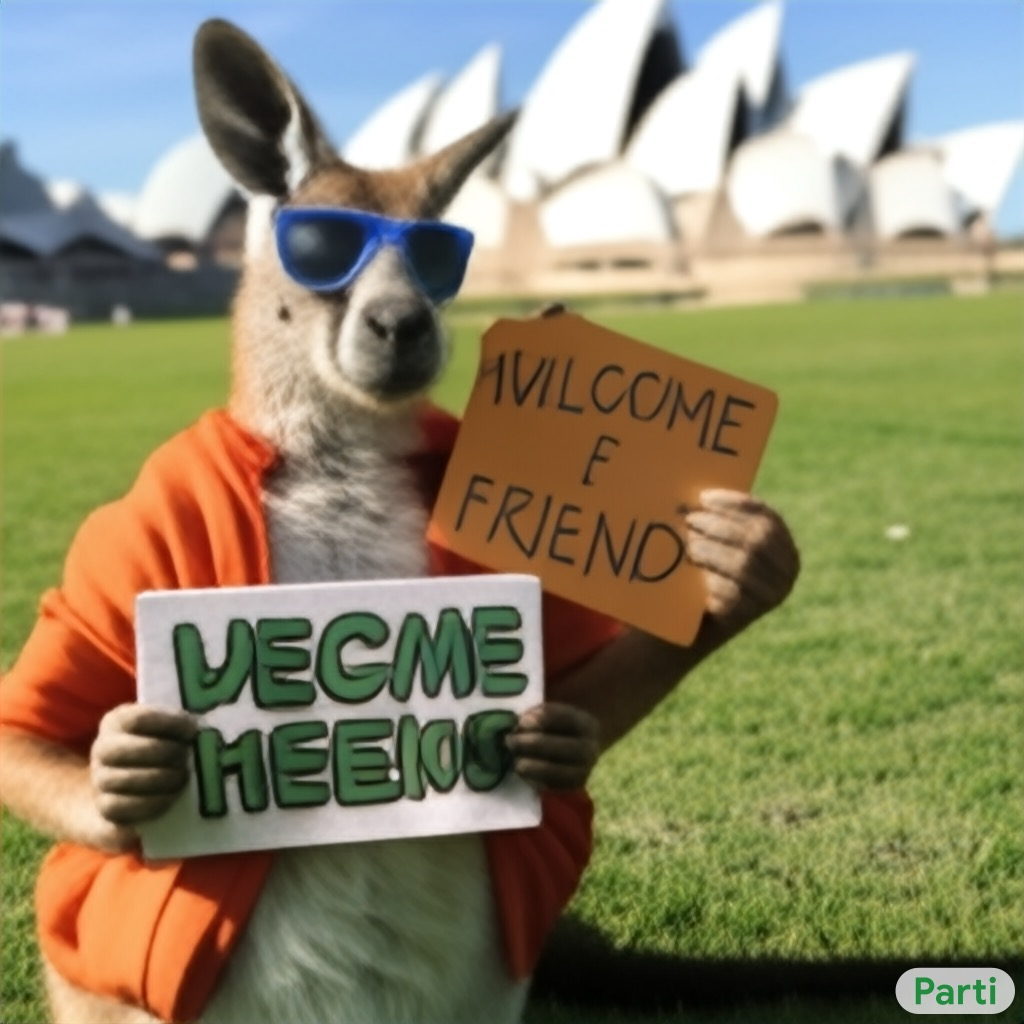
\includegraphics[width=0.24\textwidth]{figures/scaling_comparison/kangaroo_2.jpg} &
        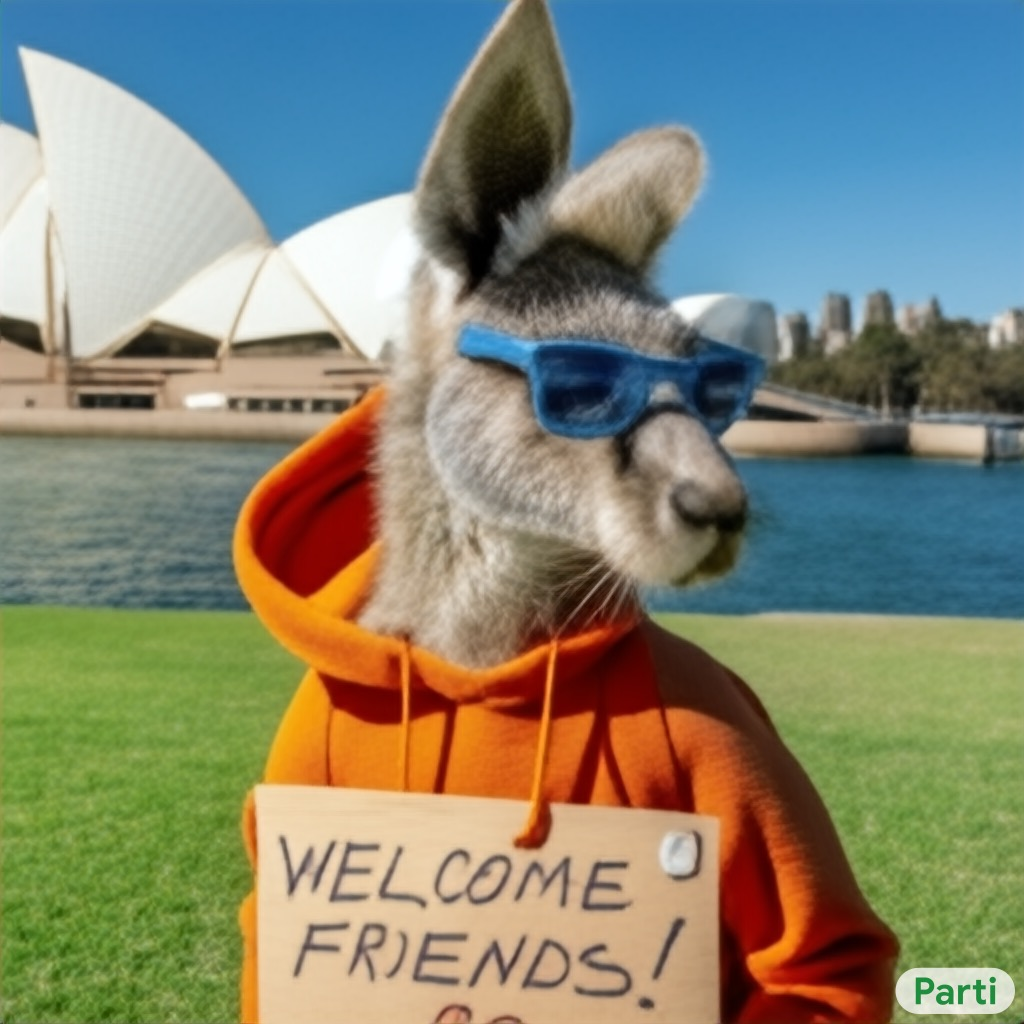
\includegraphics[width=0.24\textwidth]{figures/scaling_comparison/kangaroo_3.jpg}\vspace{1mm} \\
        \multicolumn{4}{c}{\small A portrait photo of a kangaroo wearing an orange hoodie and blue sunglasses standing on the grass} \\
        \multicolumn{4}{c}{\small in front of the Sydney Opera House holding a sign on the chest that says Welcome Friends!}\vspace{3mm}\\

        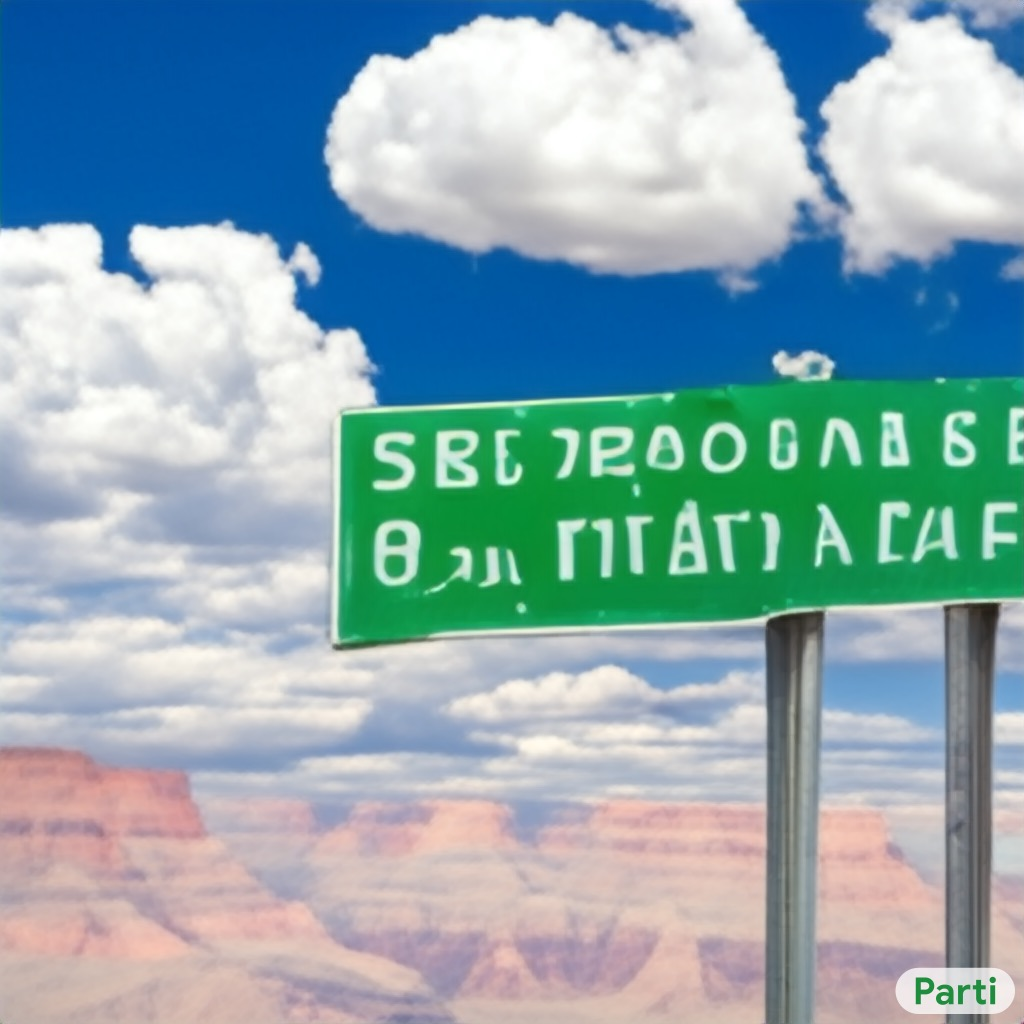
\includegraphics[width=0.24\textwidth]{figures/scaling_comparison/dl_0.jpg} &
        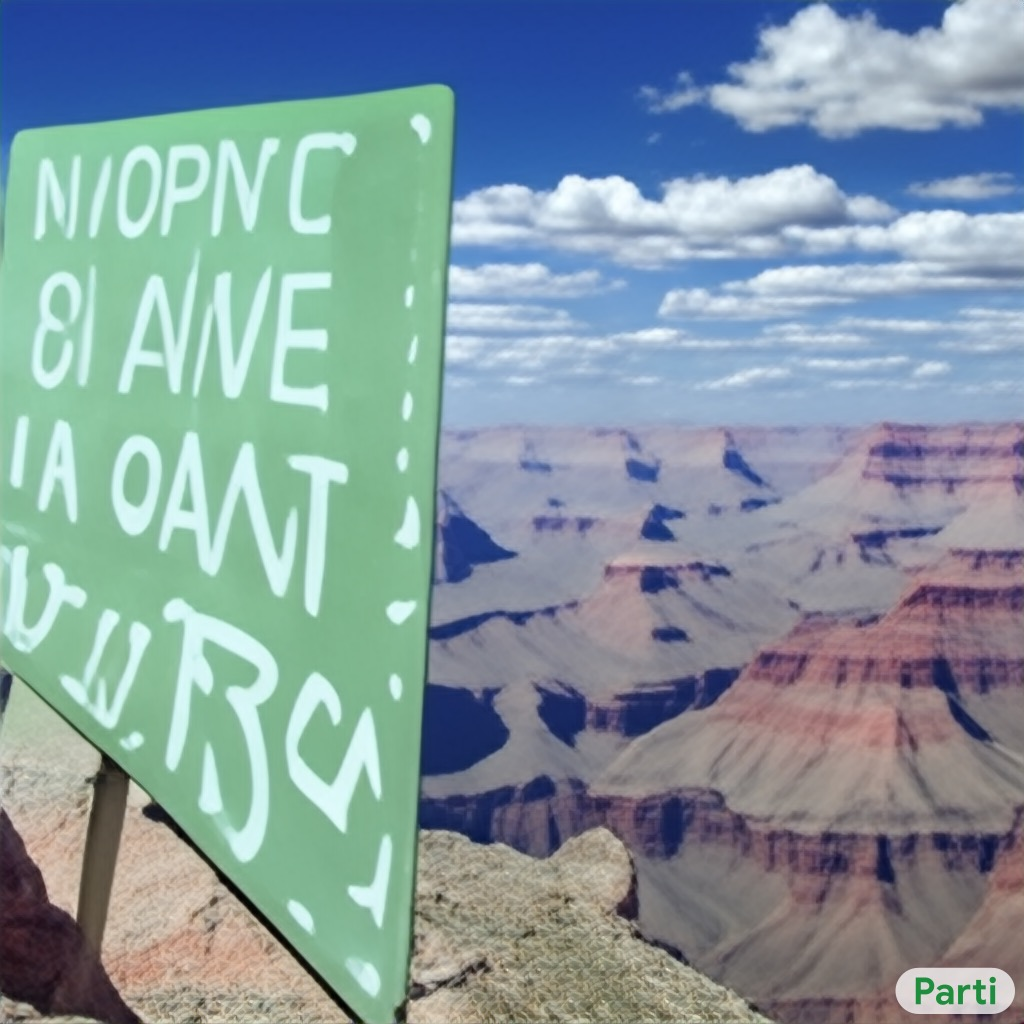
\includegraphics[width=0.24\textwidth]{figures/scaling_comparison/dl_1.jpg} &
        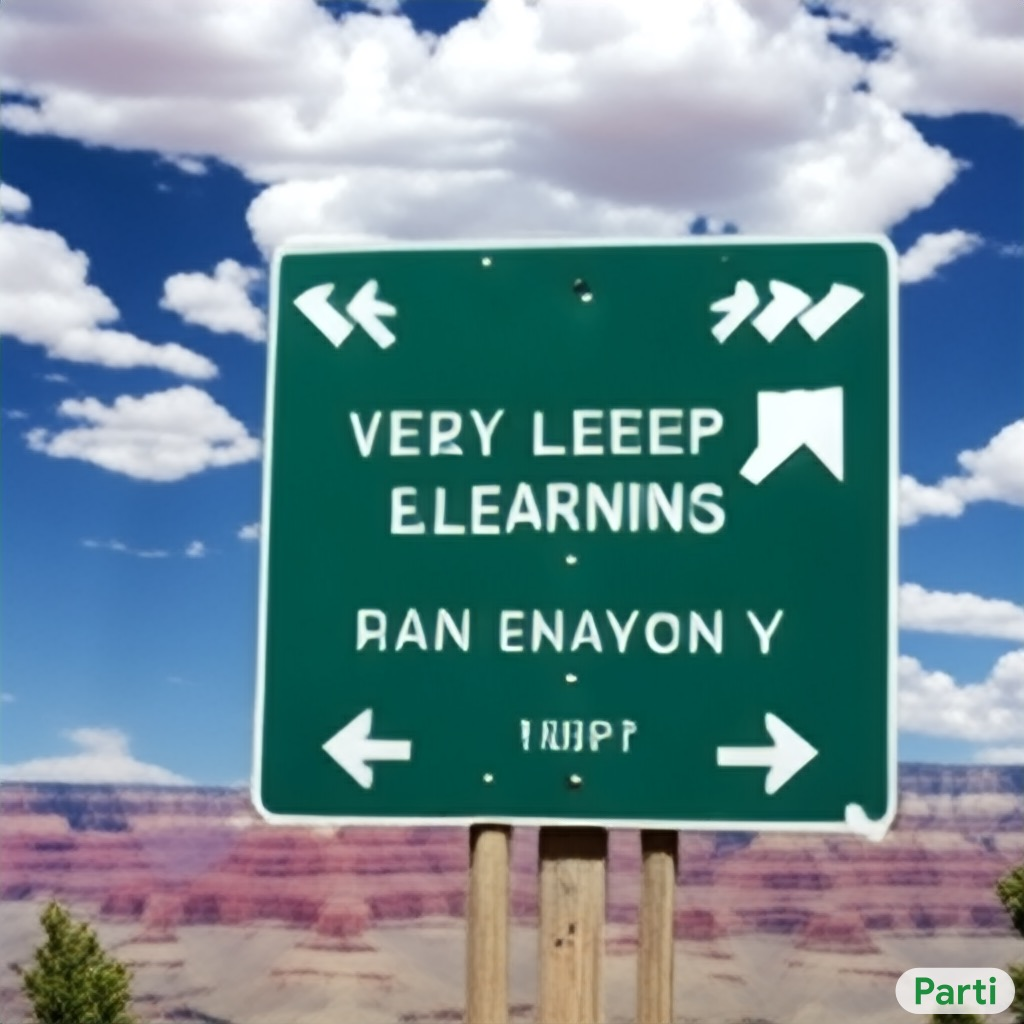
\includegraphics[width=0.24\textwidth]{figures/scaling_comparison/dl_2.jpg} &
        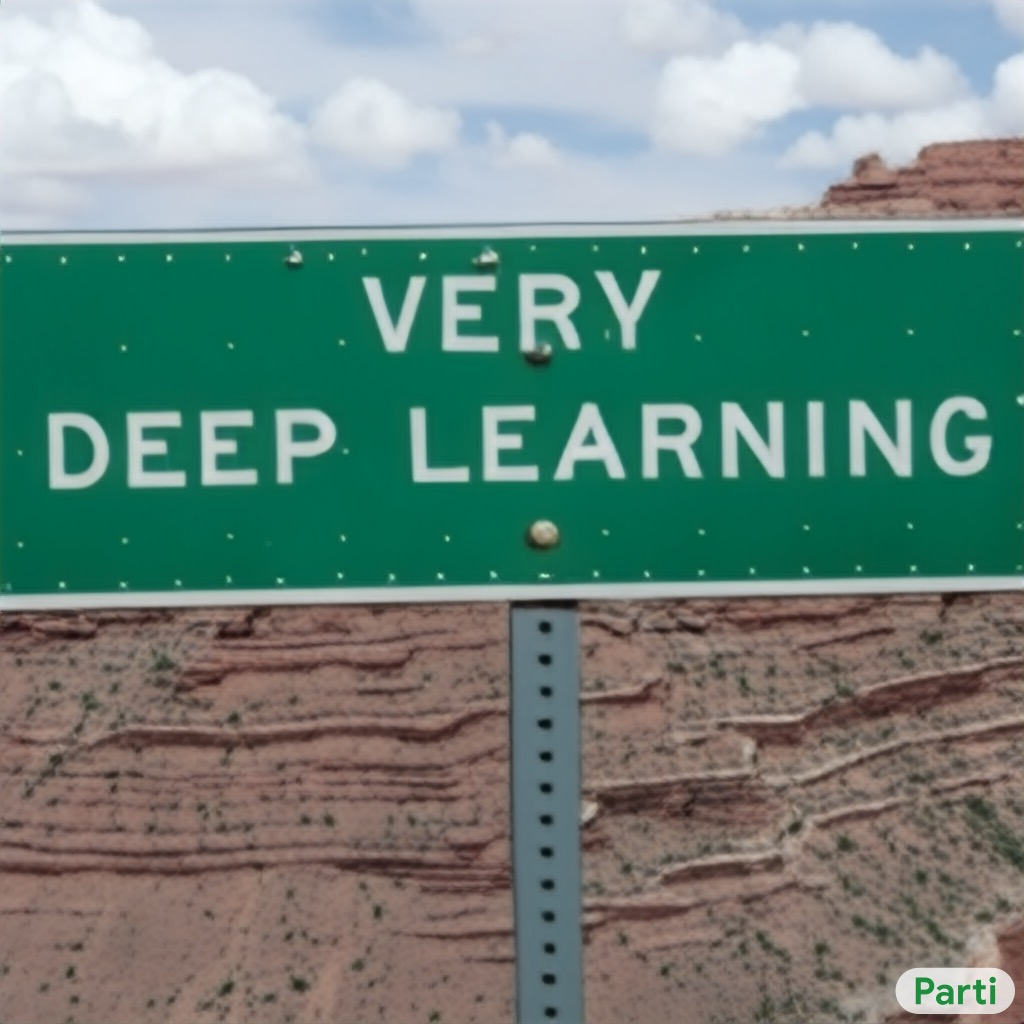
\includegraphics[width=0.24\textwidth]{figures/scaling_comparison/dl_3.jpg}\vspace{1mm} \\
        \multicolumn{4}{c}{\small A green sign that says "Very Deep Learning" and is at the edge of the Grand Canyon.}\\
        \multicolumn{4}{c}{\small Puffy white clouds are in the sky.}\vspace{3mm}\\

        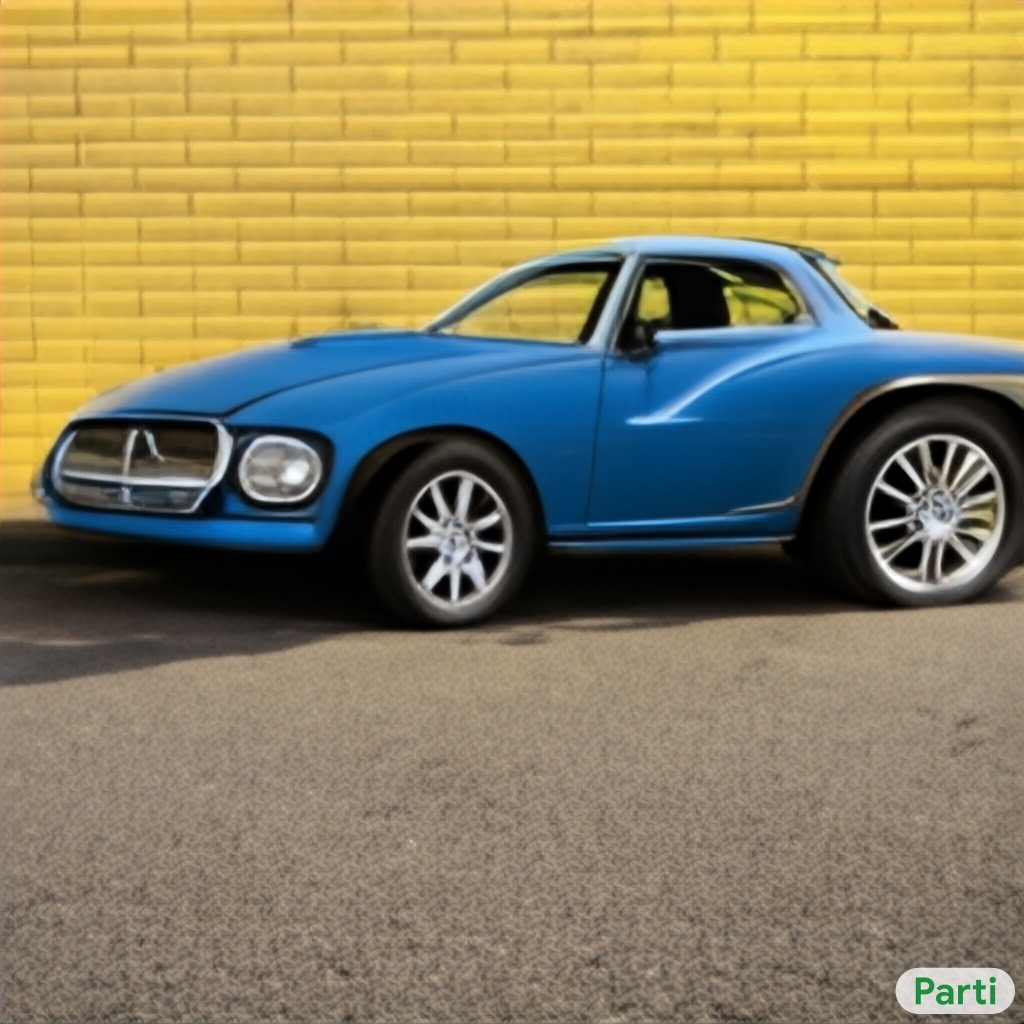
\includegraphics[width=0.24\textwidth]{figures/scaling_comparison/p356_0.jpg} &
        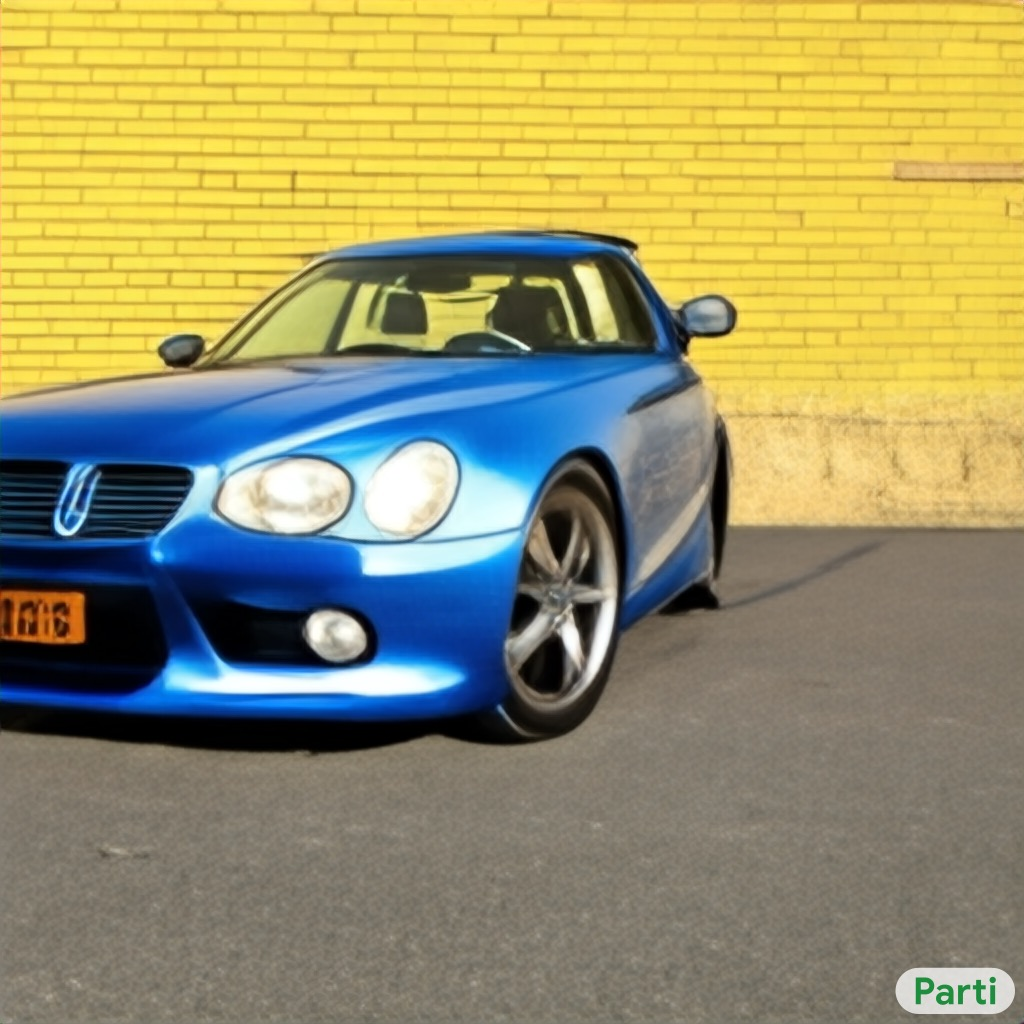
\includegraphics[width=0.24\textwidth]{figures/scaling_comparison/p356_1.jpg} &
        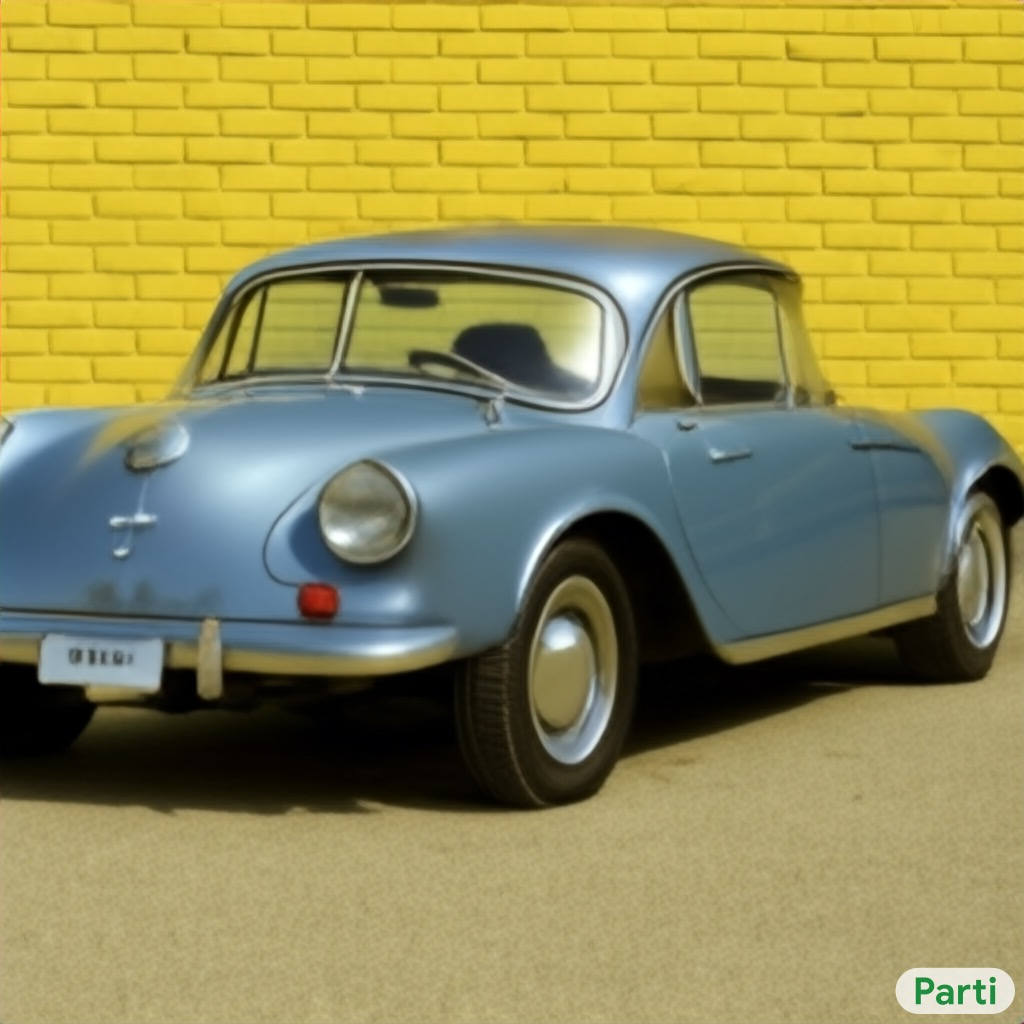
\includegraphics[width=0.24\textwidth]{figures/scaling_comparison/p356_2.jpg} &
        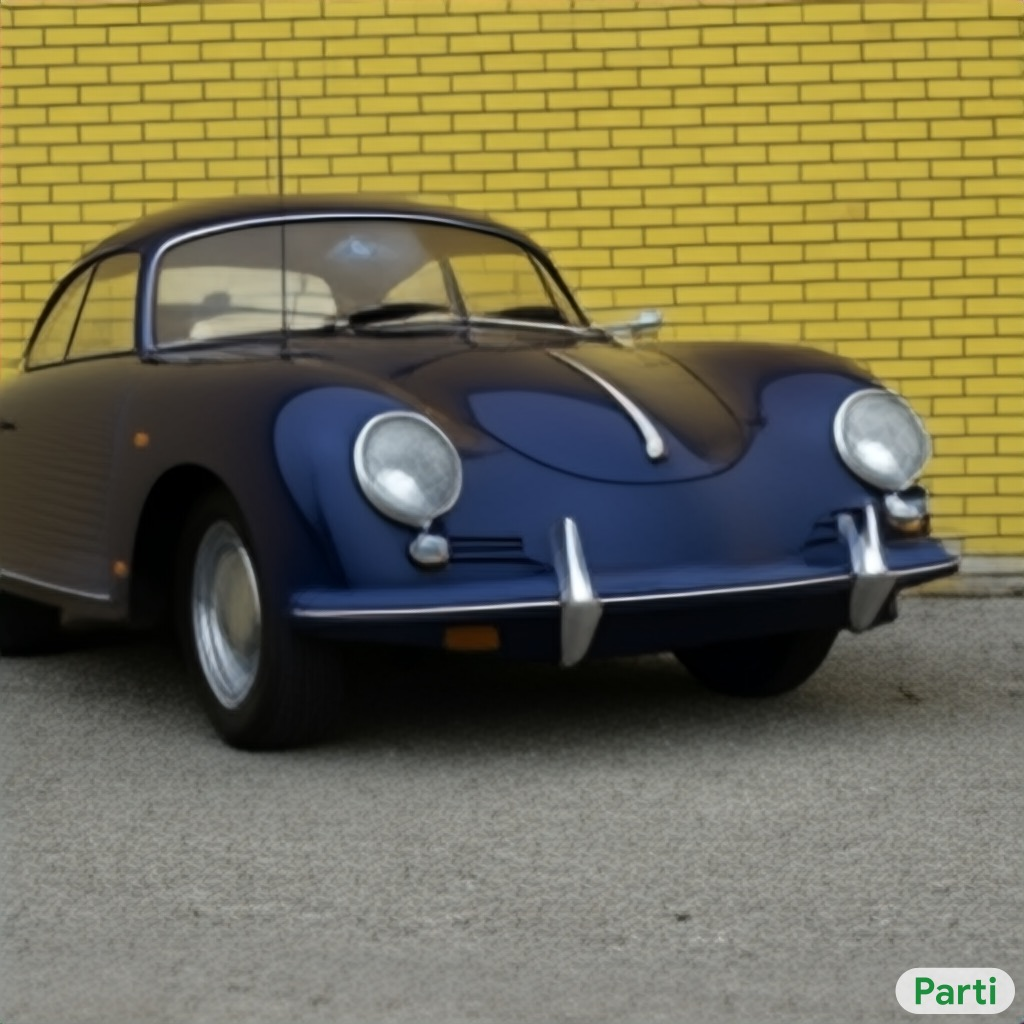
\includegraphics[width=0.24\textwidth]{figures/scaling_comparison/p356_3.jpg}\vspace{1mm} \\
        \multicolumn{4}{c}{\small A blue Porsche 356 parked in front of a yellow brick wall.}\vspace{3mm}\\

        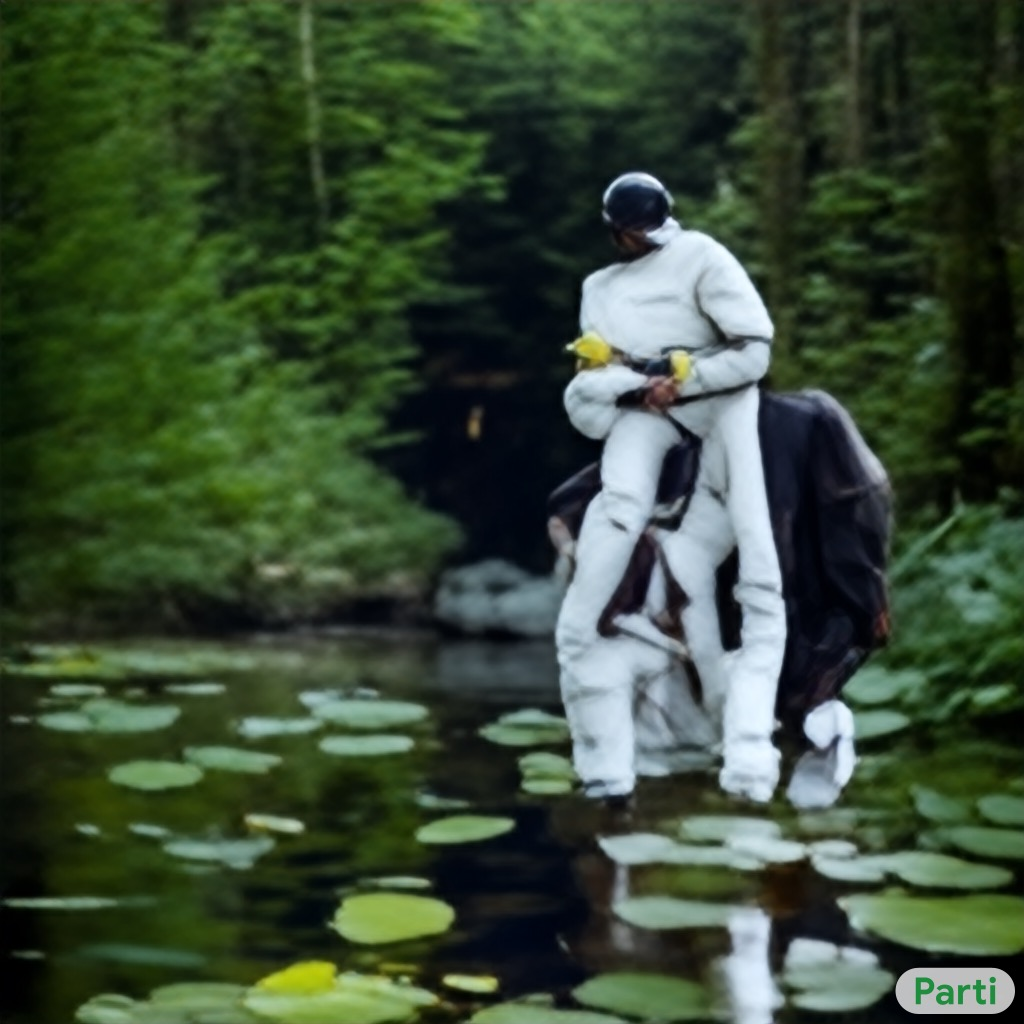
\includegraphics[width=0.24\textwidth]{figures/scaling_comparison/astronaut_0.jpg} &
        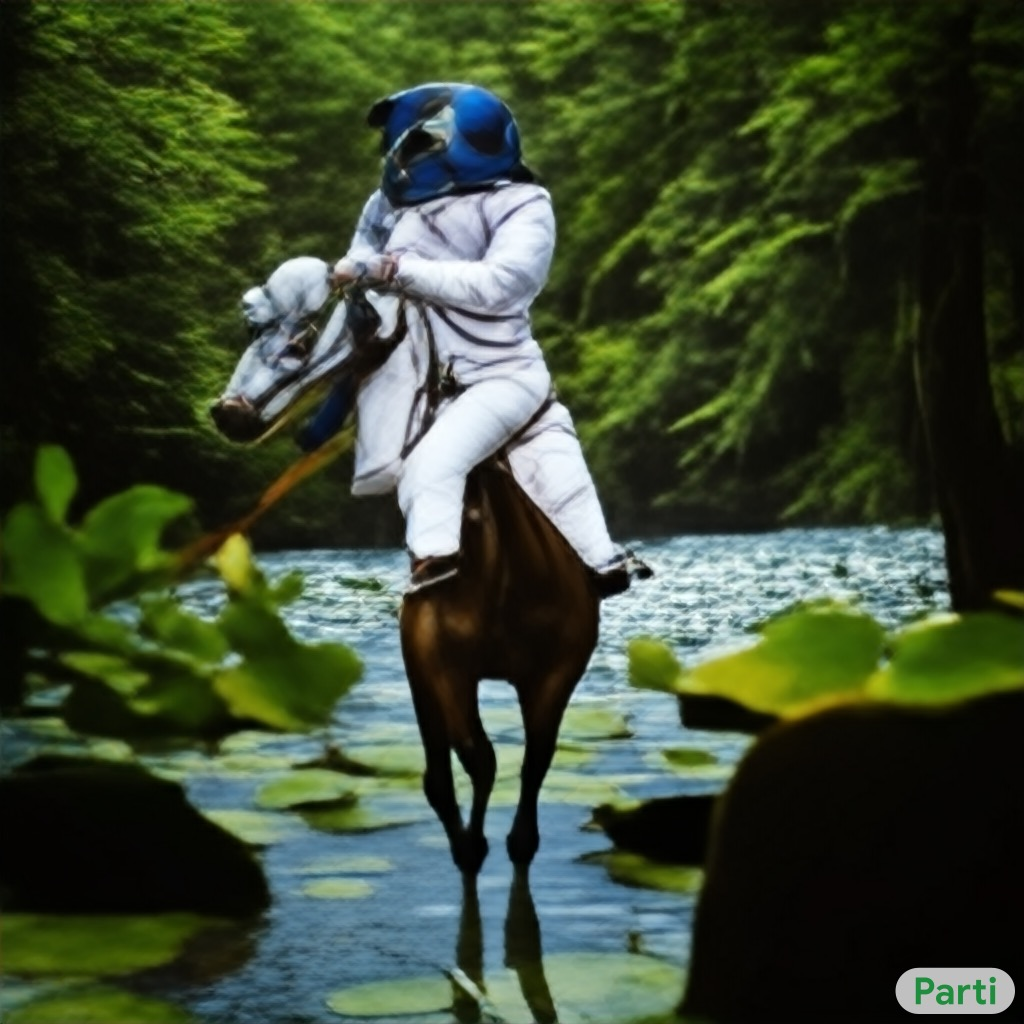
\includegraphics[width=0.24\textwidth]{figures/scaling_comparison/astronaut_1.jpg} &
        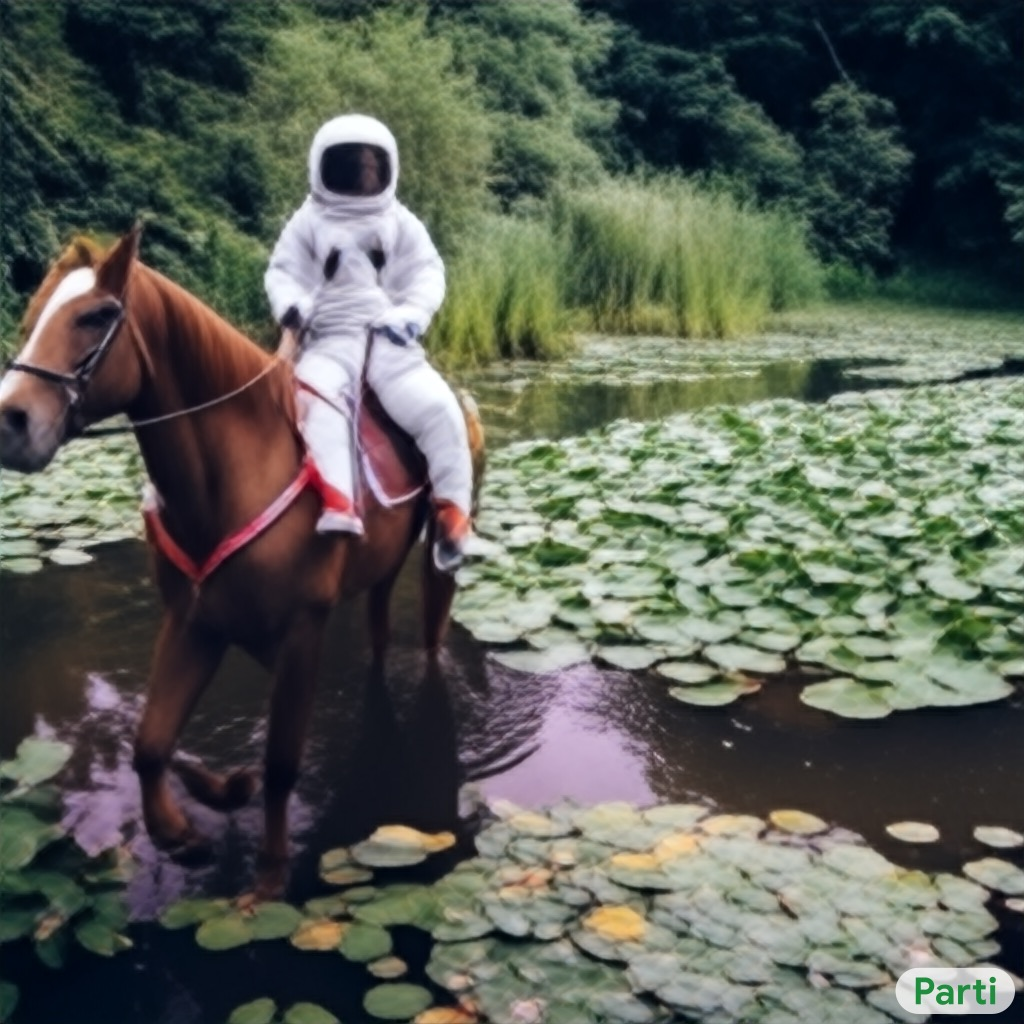
\includegraphics[width=0.24\textwidth]{figures/scaling_comparison/astronaut_2.jpg} &
        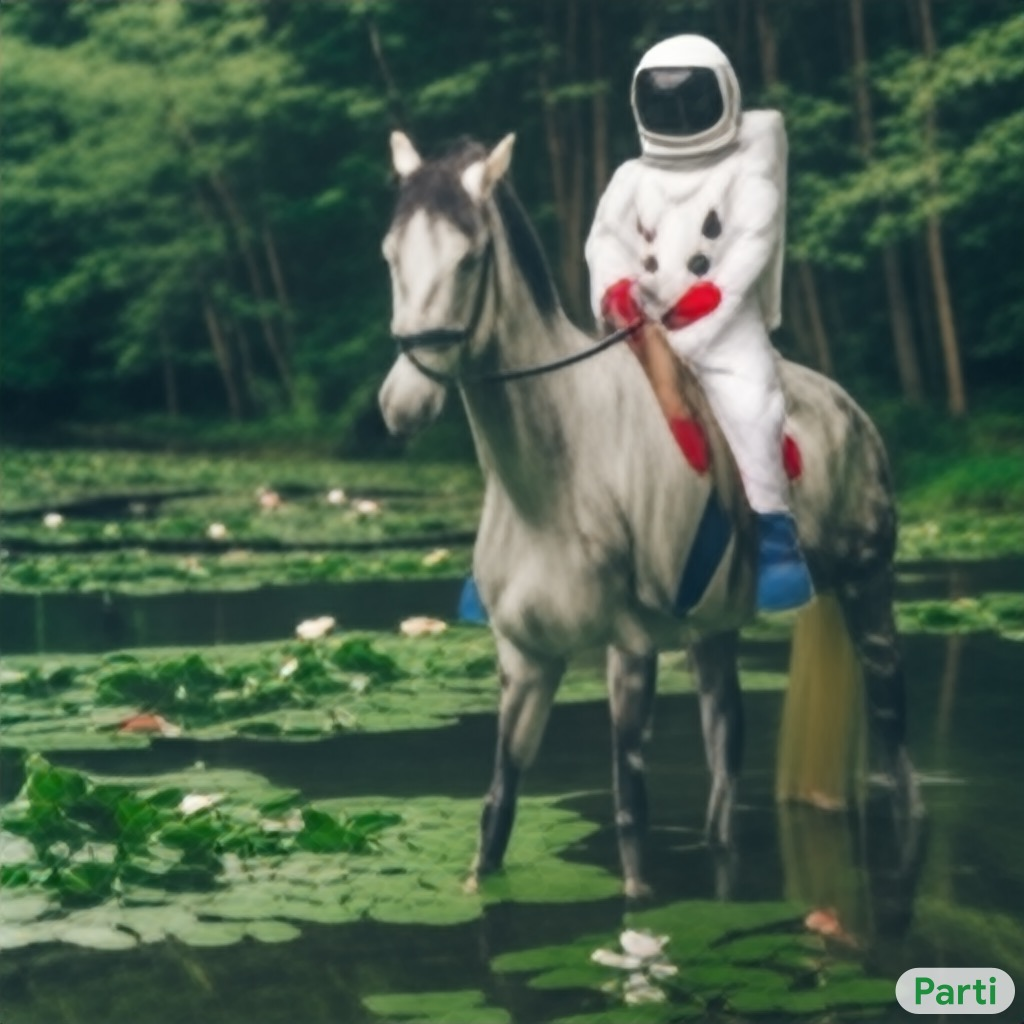
\includegraphics[width=0.24\textwidth]{figures/scaling_comparison/astronaut_3.jpg}\vspace{1mm} \\
        \multicolumn{4}{c}{\small A photo of an astronaut riding a horse in the forest. There is a river in front of them with water lilies.}\vspace{3mm}\\

        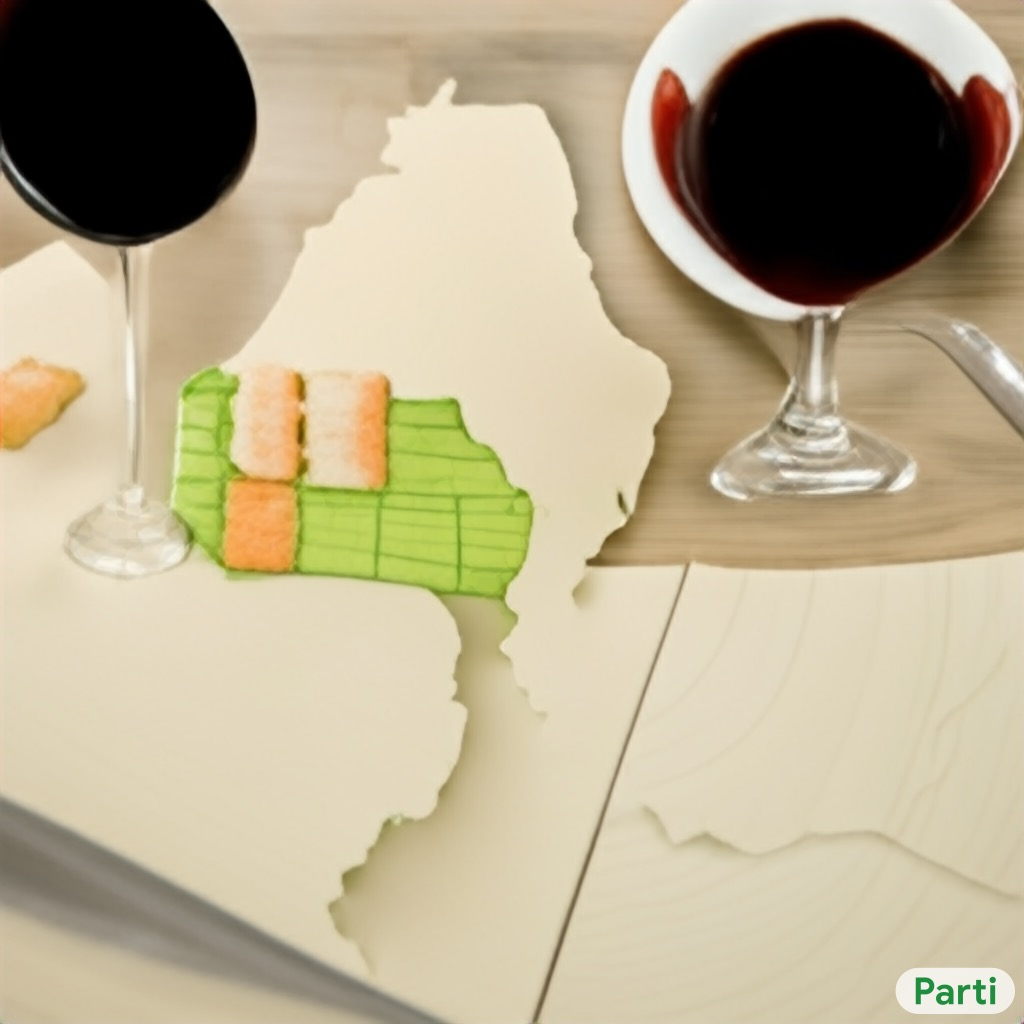
\includegraphics[width=0.24\textwidth]{figures/scaling_comparison/map_0.jpg} &
        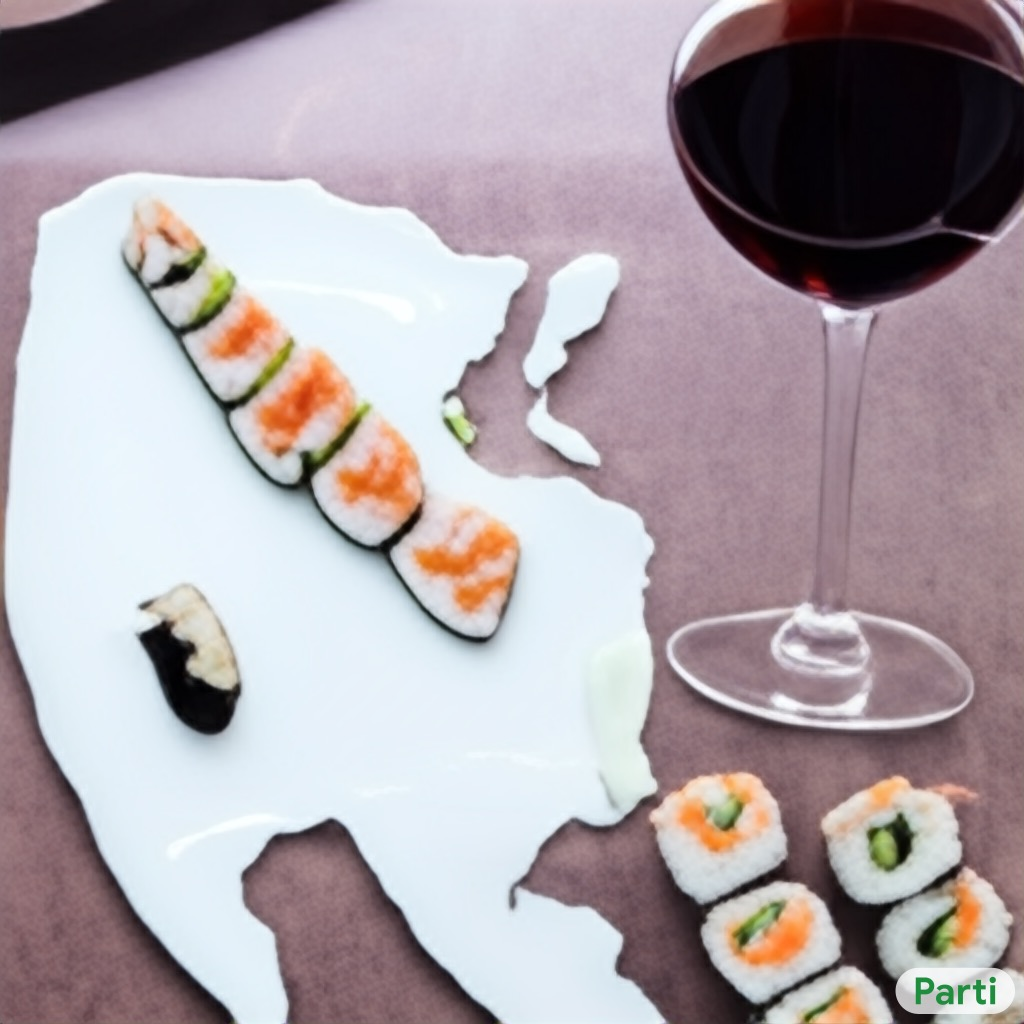
\includegraphics[width=0.24\textwidth]{figures/scaling_comparison/map_1.jpg} &
        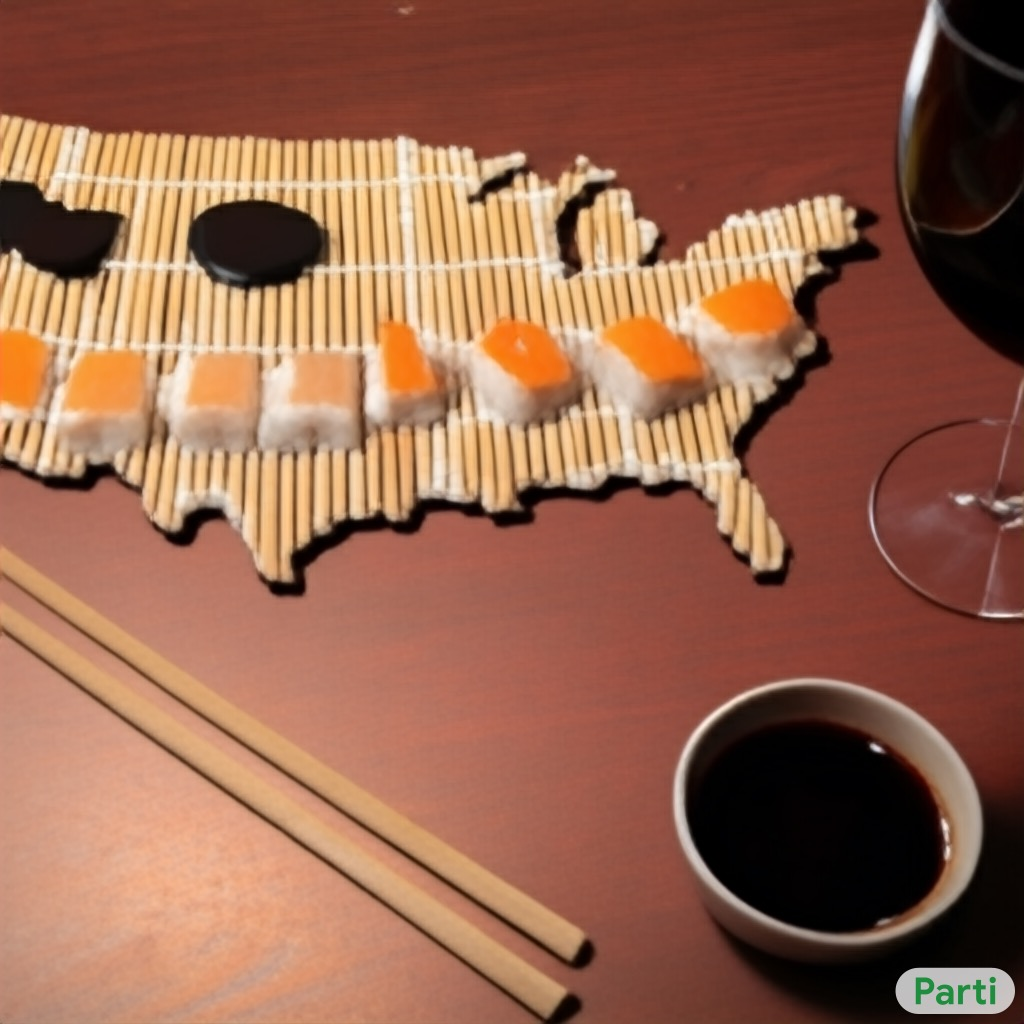
\includegraphics[width=0.24\textwidth]{figures/scaling_comparison/map_2.jpg} &
        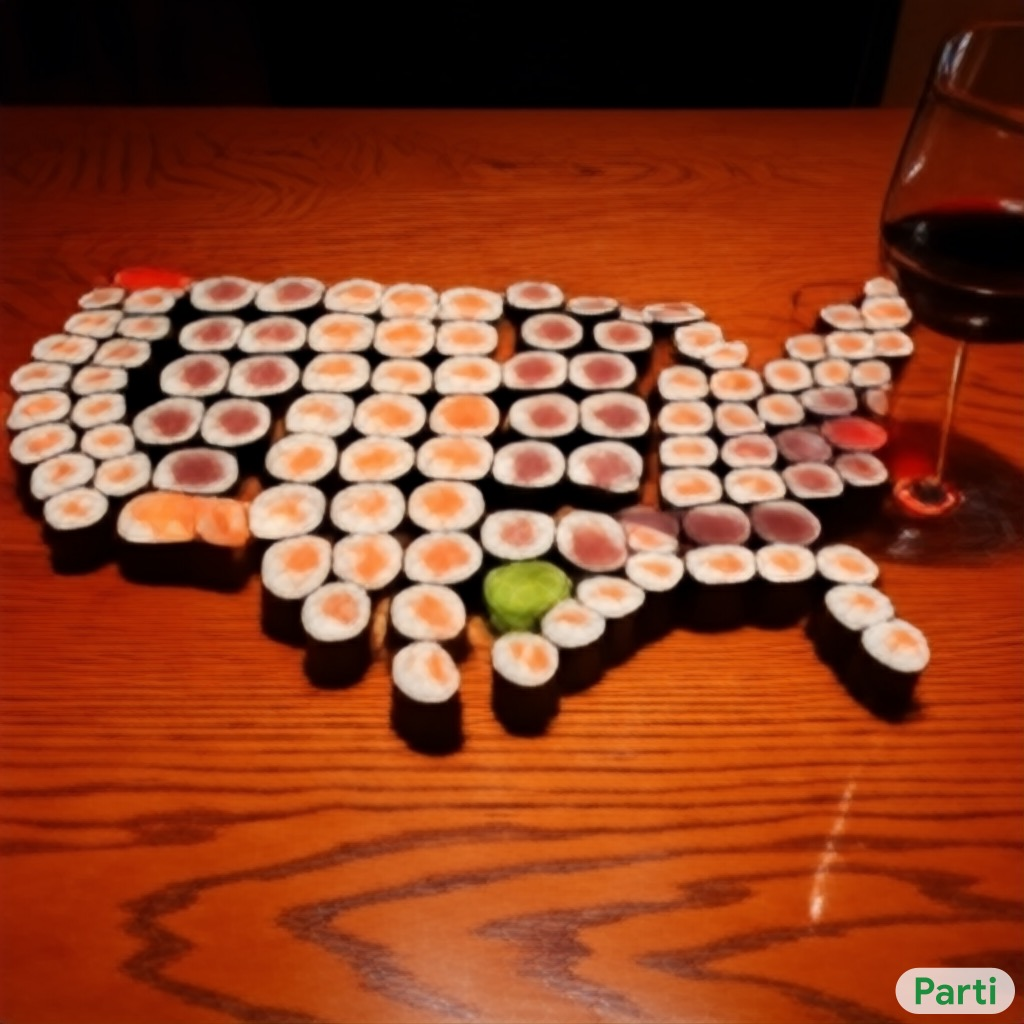
\includegraphics[width=0.24\textwidth]{figures/scaling_comparison/map_3.jpg}\vspace{1mm} \\
        \multicolumn{4}{c}{\small A map of the United States made out of sushi. It is on a table next to a glass of red wine.} \\
    \end{tabular} 
    \caption{Qualitative comparison of top-1 images sampled from \bdraw models of increasing sizes (350M, 750M, 3B, 20B). All \bdraw models sample 16 images per text prompt and rerank using the same CoCa model described in Section~\ref{secs:sampling_cf_coca}. We use prompts in the \bcpa{} benchmark (Section~\ref{secs:bcp}) to test \bcpstyle{World Knowledge}, \bcpstyle{Fine-grained Detail}, and \bcpstyle{Writing \& Symbols.}
    }
    \label{figs:scaling_comparison}
    \vspace{-0.15in}
\end{figure}